% Figura: de onde vem o N de uma condição de teste (2026-11-04).
%   (a) pior caso (símbolo 6) e (b) melhor caso (símbolo 13): as 8 posições de um
%       intervalo de T_c = 8 símbolos (TDLB100-400) que contêm o símbolo.
%   A antiga parte (a), o PRB em um slot, virou a Figura fig:prb-dmrs (fig-prb-dmrs.tex).
%   Contagens geradas em Python (DM-RS em {2,3,10,11}, slots contínuos, L = 8).
%   Cores repetidas de fig-prb-dmrs.tex, para a figura não depender da ordem.
\definecolor{dmrsfill}{HTML}{CDE2FB}
\definecolor{winblue}{HTML}{0D366B}
\definecolor{inksec}{HTML}{52514E}
\begin{figure}[htbp]
\caption{Intervals of duration $T_c$ that contain a data symbol, and their DM-RS REs per PRB, in the TDLB100-400 condition.}
\label{fig:dmrs-n}
\vspace{4pt} % a classe zera o espaço entre a caption e a figura
\centering
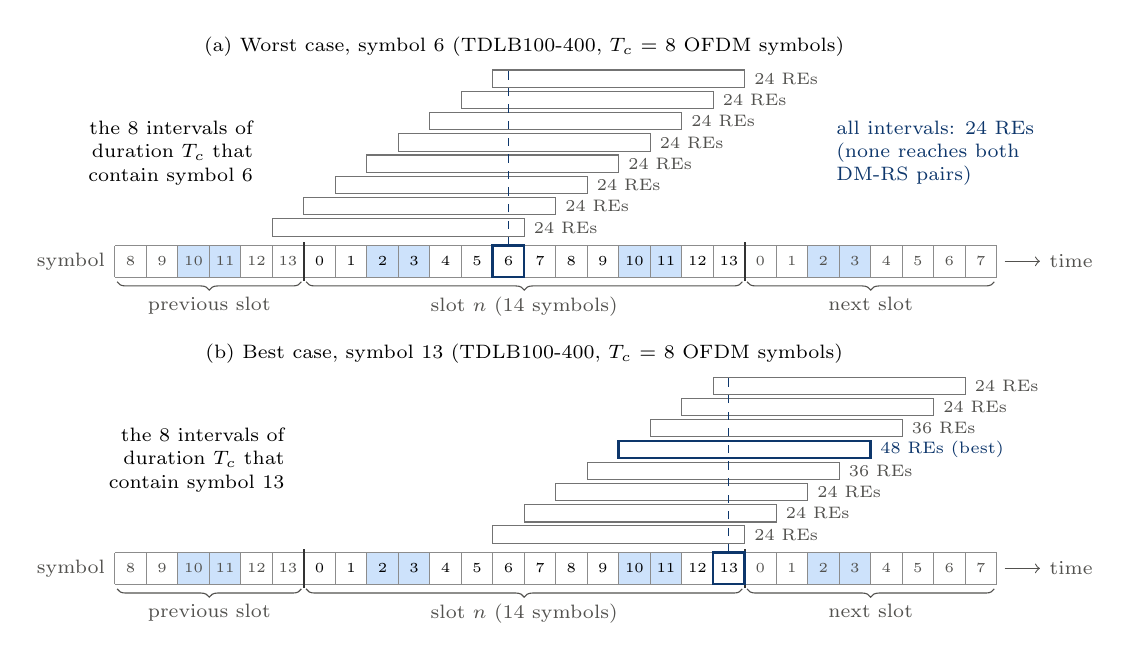
\begin{tikzpicture}[font=\fontsize{7}{8.4}\selectfont]
% ------------------------------------------------------------------ (a) e (b)
% (a) pior caso, símbolo 6; (b) melhor caso, símbolo 13. TDLB100-400, T_c = 8 símbolos.
%     Cada barra é uma posição de um intervalo de duração T_c que contém o símbolo.
%     Contagens geradas em Python: símbolo 6 -> todas 24; símbolo 13 -> 24 24 24 36 48 36 24 24.
\def\u{0.40}
\begin{scope}[shift={(0,0)}]
  \foreach \x in {-4,-3,2,3,10,11,16,17}
    \fill[dmrsfill] (\x*\u,0) rectangle ++(\u,\u);
  \foreach \x in {-6,...,22}
    \draw[black!45, line width=0.3pt] (\x*\u,0) -- (\x*\u,\u);
  \draw[black!45, line width=0.3pt] (-6*\u,0) -- (22*\u,0) (-6*\u,\u) -- (22*\u,\u);
  \draw[black!80, line width=0.6pt] (0,-0.05) -- (0,\u+0.05) (14*\u,-0.05) -- (14*\u,\u+0.05);
  \foreach \x/\l in {-6/8,-5/9,-4/10,-3/11,-2/12,-1/13,14/0,15/1,16/2,17/3,18/4,19/5,20/6,21/7}
    \node[inksec, font=\fontsize{5.5}{6}\selectfont] at (\x*\u+\u/2,\u/2) {\l};
  \foreach \s in {0,...,13}
    \node[font=\fontsize{5.5}{6}\selectfont] at (\s*\u+\u/2,\u/2) {\s};
  \node[inksec, left] at (-6*\u,\u/2) {symbol};
  \draw[inksec, ->] (22*\u+0.1,\u/2) -- ++(0.45,0) node[right] {time};
  \draw[decorate, decoration={brace, mirror, amplitude=3pt}, inksec, line width=0.4pt] (-6*\u+0.03,-0.06) -- (-0.03,-0.06) node[midway, below=2pt] {previous slot};
  \draw[decorate, decoration={brace, mirror, amplitude=3pt}, inksec, line width=0.4pt] (0.03,-0.06) -- (14*\u-0.03,-0.06) node[midway, below=2pt] {slot $n$ (14 symbols)};
  \draw[decorate, decoration={brace, mirror, amplitude=3pt}, inksec, line width=0.4pt] (14*\u+0.03,-0.06) -- (22*\u-0.03,-0.06) node[midway, below=2pt] {next slot};
  \draw[winblue, line width=0.9pt] (6*\u,0) rectangle ++(\u,\u);
  \draw[black!55, line width=0.4pt] (-1*\u,0.520) rectangle (7*\u,0.740);
  \node[inksec, right, font=\fontsize{6}{7}\selectfont] at (7*\u,0.630) {24 REs};
  \draw[black!55, line width=0.4pt] (0*\u,0.790) rectangle (8*\u,1.010);
  \node[inksec, right, font=\fontsize{6}{7}\selectfont] at (8*\u,0.900) {24 REs};
  \draw[black!55, line width=0.4pt] (1*\u,1.060) rectangle (9*\u,1.280);
  \node[inksec, right, font=\fontsize{6}{7}\selectfont] at (9*\u,1.170) {24 REs};
  \draw[black!55, line width=0.4pt] (2*\u,1.330) rectangle (10*\u,1.550);
  \node[inksec, right, font=\fontsize{6}{7}\selectfont] at (10*\u,1.440) {24 REs};
  \draw[black!55, line width=0.4pt] (3*\u,1.600) rectangle (11*\u,1.820);
  \node[inksec, right, font=\fontsize{6}{7}\selectfont] at (11*\u,1.710) {24 REs};
  \draw[black!55, line width=0.4pt] (4*\u,1.870) rectangle (12*\u,2.090);
  \node[inksec, right, font=\fontsize{6}{7}\selectfont] at (12*\u,1.980) {24 REs};
  \draw[black!55, line width=0.4pt] (5*\u,2.140) rectangle (13*\u,2.360);
  \node[inksec, right, font=\fontsize{6}{7}\selectfont] at (13*\u,2.250) {24 REs};
  \draw[black!55, line width=0.4pt] (6*\u,2.410) rectangle (14*\u,2.630);
  \node[inksec, right, font=\fontsize{6}{7}\selectfont] at (14*\u,2.520) {24 REs};
  \draw[winblue, dashed, line width=0.4pt] (6.5*\u,\u) -- (6.5*\u,2.630);
  \node[left, align=right] at (-1.3*\u,1.575) {the 8 intervals of\\duration $T_c$ that\\contain symbol 6};
  \node[winblue, right, align=left] at (16.6*\u,1.575) {all intervals: 24 REs\\(none reaches both\\DM-RS pairs)};
  \node[above] at (7*\u,2.680) {(a) Worst case, symbol 6 (TDLB100-400, $T_c$ = 8 OFDM symbols)};
\end{scope}
\begin{scope}[shift={(0,-3.900)}]
  \foreach \x in {-4,-3,2,3,10,11,16,17}
    \fill[dmrsfill] (\x*\u,0) rectangle ++(\u,\u);
  \foreach \x in {-6,...,22}
    \draw[black!45, line width=0.3pt] (\x*\u,0) -- (\x*\u,\u);
  \draw[black!45, line width=0.3pt] (-6*\u,0) -- (22*\u,0) (-6*\u,\u) -- (22*\u,\u);
  \draw[black!80, line width=0.6pt] (0,-0.05) -- (0,\u+0.05) (14*\u,-0.05) -- (14*\u,\u+0.05);
  \foreach \x/\l in {-6/8,-5/9,-4/10,-3/11,-2/12,-1/13,14/0,15/1,16/2,17/3,18/4,19/5,20/6,21/7}
    \node[inksec, font=\fontsize{5.5}{6}\selectfont] at (\x*\u+\u/2,\u/2) {\l};
  \foreach \s in {0,...,13}
    \node[font=\fontsize{5.5}{6}\selectfont] at (\s*\u+\u/2,\u/2) {\s};
  \node[inksec, left] at (-6*\u,\u/2) {symbol};
  \draw[inksec, ->] (22*\u+0.1,\u/2) -- ++(0.45,0) node[right] {time};
  \draw[decorate, decoration={brace, mirror, amplitude=3pt}, inksec, line width=0.4pt] (-6*\u+0.03,-0.06) -- (-0.03,-0.06) node[midway, below=2pt] {previous slot};
  \draw[decorate, decoration={brace, mirror, amplitude=3pt}, inksec, line width=0.4pt] (0.03,-0.06) -- (14*\u-0.03,-0.06) node[midway, below=2pt] {slot $n$ (14 symbols)};
  \draw[decorate, decoration={brace, mirror, amplitude=3pt}, inksec, line width=0.4pt] (14*\u+0.03,-0.06) -- (22*\u-0.03,-0.06) node[midway, below=2pt] {next slot};
  \draw[winblue, line width=0.9pt] (13*\u,0) rectangle ++(\u,\u);
  \draw[black!55, line width=0.4pt] (6*\u,0.520) rectangle (14*\u,0.740);
  \node[inksec, right, font=\fontsize{6}{7}\selectfont] at (14*\u,0.630) {24 REs};
  \draw[black!55, line width=0.4pt] (7*\u,0.790) rectangle (15*\u,1.010);
  \node[inksec, right, font=\fontsize{6}{7}\selectfont] at (15*\u,0.900) {24 REs};
  \draw[black!55, line width=0.4pt] (8*\u,1.060) rectangle (16*\u,1.280);
  \node[inksec, right, font=\fontsize{6}{7}\selectfont] at (16*\u,1.170) {24 REs};
  \draw[black!55, line width=0.4pt] (9*\u,1.330) rectangle (17*\u,1.550);
  \node[inksec, right, font=\fontsize{6}{7}\selectfont] at (17*\u,1.440) {36 REs};
  \draw[winblue, line width=0.9pt] (10*\u,1.600) rectangle (18*\u,1.820);
  \node[winblue, right, font=\fontsize{6}{7}\selectfont] at (18*\u,1.710) {48 REs (best)};
  \draw[black!55, line width=0.4pt] (11*\u,1.870) rectangle (19*\u,2.090);
  \node[inksec, right, font=\fontsize{6}{7}\selectfont] at (19*\u,1.980) {36 REs};
  \draw[black!55, line width=0.4pt] (12*\u,2.140) rectangle (20*\u,2.360);
  \node[inksec, right, font=\fontsize{6}{7}\selectfont] at (20*\u,2.250) {24 REs};
  \draw[black!55, line width=0.4pt] (13*\u,2.410) rectangle (21*\u,2.630);
  \node[inksec, right, font=\fontsize{6}{7}\selectfont] at (21*\u,2.520) {24 REs};
  \draw[winblue, dashed, line width=0.4pt] (13.5*\u,\u) -- (13.5*\u,2.630);
  \node[left, align=right] at (-0.3*\u,1.575) {the 8 intervals of\\duration $T_c$ that\\contain symbol 13};
  \node[above] at (7*\u,2.680) {(b) Best case, symbol 13 (TDLB100-400, $T_c$ = 8 OFDM symbols)};
\end{scope}
\end{tikzpicture}
\vspace{4pt}
\legend{Source: the author, with the DM-RS positions of \citesp{3gpp-ts38211}. \textcolor{red}{Double-symbol DM-RS}, mapping type~A, symbols 2, 3, 10 and 11; continuous uplink. In (a) and (b), each bar is one position of an interval of duration $T_c$ that contains the marked symbol. Symbol 6 is the worst case of the slot, and symbol 13 is a best case.}
\end{figure}
